\documentclass[oneside,12pt]{report}  

% the dimensions of the page
\textheight=9.25in \topmargin=-0.5in   %See note in Chapter 8 of Sample Report about "Page scaling" option in Adobe
\textwidth=6.0in
\oddsidemargin=0.3in
\evensidemargin=0.3in  % Needed to balance even and odd pages in twoside print copy


% Useful packages
\usepackage{dtklogos}
\usepackage{amsmath}
\usepackage{textcomp}
\usepackage{listings}
\usepackage{bm}
%\usepackage[colorlinks=true,pagebackref,linkcolor=blue]{hyperref}
\usepackage{amsfonts}
\usepackage{amsthm}
\usepackage{amsmath}
\usepackage{algorithm}
\usepackage{algorithmic}
\usepackage{graphicx, subfigure}
\usepackage{caption}
\usepackage{excludeonly}

\usepackage{graphicx} 

%\usepackage{doc}
%% Following sets up logic and formatting for conditional twoside copying
%\usepackage{ifthen, color, fancyvrb}
%\usepackage{nextpage}\pagestyle{plain}
%\newcommand\myclearpage{\cleartooddpage
%  [\thispagestyle{empty}]
%  }

\DeclareMathOperator*{\argmin}{arg\ min}
\DeclareMathOperator*{\sign}{sign}

% Note special alternative codes for using TWO bibliographies; see cautionary note in
\DeclareGraphicsExtensions{ps,eps,PNG,png}

% Theorem-like command definitions:
\newtheorem{theorem}{Theorem}[chapter]
\newtheorem{lemma}{Lemma}[chapter]
\newtheorem{definition}{Definition}  % Note, this italicizes everything

% Print the chapter and sections in the toc
\setcounter{tocdepth}{1}

% Specify which files to typeset for this run (note that overall pagination is preserved)
%\includeonly{chapter1, chapter2}
% Specify which files NOT to typeset for this run (note that overall pagination is preserved)
%\excludeonly{}

% Groundwork for allowing double-sided copying with blank versos
\def\prefacesection#1{
\chapter*{#1}
\addcontentsline{toc}{chapter}{#1}
}


\lstset{
basicstyle=\footnotesize\ttfamily,
language=R,
upquote=true,
breakatwhitespace=true,
columns=fullflexible,
keepspaces,
%numbers=none,
tabsize=3,
frame=bottomline,
framextopmargin=50pt,
showstringspaces=false,
extendedchars=true
}

\begin{document}


\def\thefootnote{\fnsymbol{footnote}}

\thispagestyle{empty}

% The numbers below controls the amount of space between the following sections
\def\shiftdowna{0.32in}  % Adjust for balance
\def\shiftdownb{0.22in}  % Adjust for balance

% Set up the boiler plate at the top of the page

\begin{center}
\textbf{{\large Mathematical Modeling and Consulting }}\\

\vspace \shiftdowna

\includegraphics[width=0.5\textwidth]{jhu.png}\\

% Home Department
\vspace \shiftdowna
\underline {Sponsor}\\ 
\vspace{5pt}
\textbf{\large McDonald's Corporation} \\
\vspace\shiftdowna
\textbf{{Final Report}}

% TITLE
\vspace \shiftdowna
\textbf{{\Large How Much Ice Do You Need?}}

% STUDENTS
\vspace{0.35in}
\underline {Team Members}\\
\vspace{5pt}
Yen Theng Tan \\
\texttt{yen@jhu.edu} \\
\vspace{10pt}
Joyce Tan \\
\texttt{jtan21@jhu.edu}

% INSTRUCTOR
\vspace \shiftdownb
\underline {Academic Mentor} \\
\vspace{5pt}
\text{Dr.~N.~.H.~Lee}\\
\texttt{nhlee@jhu.edu}

% Consultants
%\vspace \shiftdownb 
%\underline {Consultant}\\
%\vspace{5pt}
%Jason Bourne\\

% DATE
\vspace \shiftdowna
Date: Last Complied on \today

\end{center}

\vfill  %Fill page to force following note to bottom

% Begin ABSTRACT
\ifthenelse{\boolean{@twoside}}{\myclearpage}{}
\prefacesection{Abstract}

McDonald's Corporation is the world's largest chain of hamburger fastfood restaurants, and selling soft drinks is a significant portion of McDonald's business. The server is not accustomed to putting much thought in measuring the amount of ice put in the cup. This often results in a overly diluted, overly concentrated or warmer drink for the customer. Our task is to provide a suggestion for the optimal amount of ice for soda, such that the average consumer will be most satisfied. We approach this problem by first creating an experiment that measures consumer preferences to the amount of ice in a large McDonald's cup, and different points in time after the ice is initially mixed with the soda. The collected data is statistically analyzed to give us an idea of the optimal amount of ice to be added. Secondly, we calculate the different temperatures and the amount of dilution of the resulting drink, using specific heat capacities of soda and ice. This can be used complementary to our first experiment to provide more theoretical reasonings behind any trends or conclusions. 


% Begin ACKNOWLEDGMENTS
\ifthenelse{\boolean{@twoside}}{\myclearpage}{}
\prefacesection{Acknowledgments}

\vspace{12pt}
We would like to acknowledge McDonald's Corporation for their support of our project. 

\vspace{12pt}
We would also like to acknowledge Dr.~N.~.H.~Lee, our course professor in the Mathematical Modeling and Consulting class at Johns Hopkins University, without whom we would not have had the tools and feedback necessary to complete this project. 

% Table of contents, List of Figures, and List of Tables.
\ifthenelse{\boolean{@twoside}}{\myclearpage}{}
\tableofcontents

%\ifthenelse{\boolean{@twoside}}{\myclearpage}{}
%\listoffigures

\ifthenelse{\boolean{@twoside}}{\myclearpage}{}
\listoftables


\renewcommand{\thefootnote}{\arabic{footnote}}
\setcounter{footnote}{0}

\ifthenelse{\boolean{@twoside}}{\myclearpage}{}
%\include{A_Introduction}

\ifthenelse{\boolean{@twoside}}{\myclearpage}{}
\prefacesection{Introduction}

McDonald's Corporation is the world's largest chain of hamburger fastfood restaurants, serving around 68 million customers daily in 119 countries. Mcdonald's primarily sells hamburgers, cheeseburgers, chicken, French fries, breakfast items, soft drinks, milkshakes and desserts. 
No meal is complete without a drink; and from Diet Coke to low-fat milk to fresh-brewed, hot coffee, McDonald's serves many different varieties of beverages. 
\\* Given that soft drinks are normally assumed to be the perfect accompaniment to a fast food meal, their temperature is also essential to the overall satisfaction of the consumer. We have been tasked by McDonald's to find the optimal amount of ice to put into their standard large size cups, and the provide them with data on consumer satisfaction as time elapses. 

%\include{B_ProblemStatement}

\ifthenelse{\boolean{@twoside}}{\myclearpage}{}
\prefacesection{Problem Statement}

Selling soft drinks is a significant portion of McDonald's business, be it as a thirst quencher, or as part of the extra value meal. The server is not accustomed to putting much thought in measuring the amount of ice put in the cup. This often results in a overly diluted, overly concentrated or overly cold drink for the customer. This is likely to lower overall customer satisfaction, since a drink is a significant complement to a meal. Thus, customers are likely to appreciate if the right amount of ice was added for optimal satisfaction.
\\* To further define this problem, the exogenous variables are the proportion of ice to put in a drink. The endogenous variable would be the resulting temperature and concentration of the drink, as we are assuming that a customer's satisfaction is affected only by the temperature and concentration of the drink.

%\include{C_TechnicalBackground}

\ifthenelse{\boolean{@twoside}}{\myclearpage}{}
\prefacesection{Technical Background}
To aid us in our analysis of the experiment that we plan to do, we will be using the Pearson's chi-squared test to test how significant our experiment results are. It tests a null hypothesis stating that the frequency distribution of certain events observe in a sample is consistent with a particular theoretical distribution. The events must be mutually exclusive and have total probability one.
\\*The Pearson's chi-squared test is used to assess two types of comparisons: tests of goodness of fit and tests of independence. Ths first step is to calculate the chi-squared statistic $ X^2$, which resembles a normalized sum of squared deviations between observed and theoretical frequencies, as shown in Equation \eqref{chisqstat}
\begin{align}
X^2 &= \sum_{i=1}^{n} {\frac{(O_{i}-E_{i})^2}{E_{i}}} \label{chisqstat}
\end{align}

where $O_{i}$ is the observed frequency of category i being chosen,
\\*$E_{i}$ is the expected theoretical frequency of category i being chosen,
\\*$n$ is the number of different categories,

\vskip3pt The second step is to determine the degrees of freedom, $d$, of that statistic, which is essentialy the number of frequencies reduced by the number of parameters of the fitted distribution. In the third step, $X^2$ is compared to the critical value of no significaned from the $\chi_{d}^{2}$ distribution, which usually gives a good approximation fo the distribution of $X^2$.
\\* By comparing the $X^2$ statistic calculated in Equation \eqref{chisqstat} to the appropiate $\chi^{2}$distribution with $d$ degrees of freedom, we will obtain a p-value. The p-value is the probability of obtaining a test statistic at least as extrememas the one that is actually observed, assuming the null hypothesis is true.
\vskip6pt $H_0$: All n categories are chosen with equal probability
\vskip3pt $H_a$: All n ncateogires are chosen with unequal probability.
\vskip6pt If the p-value is greater than a given $\alpha$, it means that the result is not that extremem assuming the null hypothesis is true. Thus, there is insufficient evidence to reject the null hypothesis that all n categories are chosen with equal probability. However, if the p-value is greater than $\alpha$, it means that observed result is too extreme assuming the null hypothesis is true. Thus, we have sufficient evidence to reject the null hypothesis and accept the alternative hypothesis.
\vskip6pt
While carrying out this test, we have to be wary of 2 statistical errors : Type I and Type II errors. Type I error is the incorrect rejection of a true null hypothesis (a false positive). The probaility of a Type I error is equal to the $\alpha$ that we use. Most statistical test usually use 0.05 for its $\alpha$. Type II error is seen as a false negative, where we accept the null hypothesis when it is not true. The probability of a Type II error is usually denoted by $\beta$. The power of a test is $1-\beta$.
\vskip6pt
There are a few assumptions in place when using the chi-squared test.
\begin{itemize}
\item The sample data is a simple random sample from a fixed distribution or population where each member of the population has an equal probability of selection. We have tried to achieve this assumption as much as possible by ensuring our sample group is as representative of the population by choosing test subjects from different backgrounds.
\item Sample size is sufficiently big. This is to avoid committing a Type II error.
\item Observations are assumed to be independent of each other. There is no correlation between the test subject's preferences in any way.


\end{itemize}


%\include{D_Methods}

\ifthenelse{\boolean{@twoside}}{\myclearpage}{}
\prefacesection{Methods}

Firstly, we have a few assumptions on hand in order to simplify this problem. We assume that the consumer's taste depends entirely on the dilution and temperature of the drink. Since both the dilution and temperature of the drink rely entirely on the ice proportion, these two values would come hand-in-hand. Also, any sample group that we use represents the population's preferences accurately. Only a similar note, the 4 different time parameterrs which we perform the experiment is sufficient to represent the overall satisfaction the customer has with the drink.
\\* We are interested in approaching this problem using 2 different methods. The first method would be experimenting with the 4 most popular types of soda at McDonald's, namely Coca Cola, Fanta Orange, Sprite and Diet Coke. Then we would experiment and gauge the satisfaction of the test subjects by experimenting with different amounts of ice to find out the optimal proportion of ice to soda. 
\\* This experiment will take place over the course of 4 days, where we will each drink will be tested on each day. For each time parameter, we will give the test subject 3 different cups (labelled A, B and C) with different ice proportions in them (40\%, 60\%, 75\%). The ice will be left in the drink for time parameter t, and then the test subject will drink the 3 different cups, and indicate their preference by ranking the cups (3 is their favorite cup, and 1 is their least favorite cup). There will be 4 similar tests done on the same day but with a different time parameter t. These 4 experiments will be scheduled an hour apart from each other, so there will be no aftereffect or bias from the previous experiment. 
The 4 different time parameters t will be t=0.5 minutes, t=2 minutes, t=5 minutes, t=30 minutes, which indicates the time elapsed after the ice is mixed with the drink. The test subject is allowed to sip the drink at time=t, assuming the ice is placed in the drink at t=0. We will tabulate the preferences of the entire sample group, and provide a conclusion about the consumer's preferred ice proportion in each soda drink.
This will be a blind test and the subject will not know which ice proportions cups A, B and C will have (it will be random every round). \pagebreak
\vspace{2pt}
\begin{table}[ h]
\centering
\begin{tabular}{ l | c|c|c }
  Ice Proportion & A  & B & C  \\
\hline  
t=0.5mins & & &\\ 
\hline  
t=2mins & & &\\ 
\hline  
t=5mins  & & &\\ 
\hline  
t=30mins & & &\\ 
\hline  
   
 \end{tabular}
\caption{Sample form each test subject will need to fill out for each drink}

\end{table}

\begin{table}[ h]
\centering
\begin{tabular}{ l | c|c|c }
  Ice Proportion & A  & B & C  \\
\hline  
t=0.5mins & 3&2 &1\\ 
\hline  
t=2mins &1 &3 &2\\ 
\hline  
t=5mins  &2 &3 &1\\ 
\hline  
t=30mins &1 &2 &3\\ 
\hline  
   
 \end{tabular}
\caption{Example of a response by a test subject}

\end{table}
\vspace{6pt}

 We would also be looking to approach this problem from an alternative, and supplementary, method. The second method would be using physics-based modeling. Utilizing the specific heat capacities of soda and ice (already found as specific values), we can calculate the different temperatures and dilution that the resulting drink will be. This would not really tell us anything about preference of the population, but if provides more of a perspective on how different ice proportions affect temperatures and dilutions. However, this is purely theoretical since it does not take into account heat loss to the environment and cup. This will be mainly a supporting tool and not used in place of the first approach.


%\include{E_Results}

\ifthenelse{\boolean{@twoside}}{\myclearpage}{}
\prefacesection{Results}
\vspace{6pt}

\begin{table}[ h]
\centering
\begin{tabular}{ l || c|c|c }
  &40\% &60\% & 75\%  \\
\hline  
t=0.5 mins & 15 & 25 & 32\\ 
\hline  
t=2 mins & 14 & 24 & 34\\ 
\hline  
t=5 mins & 14 & 27 & 31\\ 
\hline  
t=30 mins & 18 & 36 & 18\\ 
\hline  
   
 \end{tabular}

\caption{Experiment results for Coke}

\end{table}

\begin{table}[ h]
\centering
\begin{tabular}{ l || c|c|c }
  &40\% &60\% & 75\%  \\
\hline  
t=0.5 mins & 15 & 27 & 30\\ 
\hline  
t=2 mins & 20 & 19 & 33\\ 
\hline  
t=5 mins & 14 & 29 & 29\\ 
\hline  
t=30 mins & 17 & 30 & 25\\ 
\hline  
   
 \end{tabular}

\caption{Experiment results for Sprite}

\end{table}
\begin{table}[ h]
\centering
\begin{tabular}{ l || c|c|c }
  &40\% &60\% & 75\%  \\
\hline  
t=0.5 mins & 15 & 23 & 34\\ 
\hline  
t=2 mins & 19 & 23 & 30\\ 
\hline  
t=5 mins & 18 & 27 & 27\\ 
\hline  
t=30 mins & 12 & 35 & 25\\ 
\hline  
   
 \end{tabular}

\caption{Experiment results for Fanta Orange}

\end{table}
\begin{table}[ h]
\centering
\begin{tabular}{ l || c|c|c }
  &40\% &60\% & 75\%  \\
\hline  
t=0.5 mins & 15 & 24 & 33\\ 
\hline  
t=2 mins & 21& 19 & 32\\ 
\hline  
t=5 mins & 16 & 24 & 32\\ 
\hline  
t=30 mins & 18 & 22& 32\\ 
\hline  
   
 \end{tabular}

\caption{Experiment results for Diet Coke}

\end{table}
\begin{table}[ h]
\centering
\begin{tabular}{ l || c|c}
 Volume of ice to volume of soda &Dilution &Temperature (Celsius) \\
\hline  
1/10 & 0.09&16.2\\ 
\hline  
1/8 & 0.11&14.3\\ 
\hline 
1/6 & 0.15&11.2\\ 
\hline 
1/5 & 0.18&8.8\\ 
\hline 
1/4 & 0.23&5.5\\ 
\hline    
\end{tabular}
\caption{Calculated dilution and temperature for difference ice volumes}
\end{table}

%\include{F_Analysis}

\ifthenelse{\boolean{@twoside}}{\myclearpage}{}
\prefacesection{Analysis}

We run the Pearson's chi-squared test on the results that we have obtain with the following null hypothesis.
\vskip6pt $H_0$: The 3 different proportions are desired to an equal extent by the population.
\vskip3pt $H_a$: The 3 different proportions are not desired to an equal extent by the population.
\vskip6pt

Since there are 72 points to be awarded (12 test subjects can give 6 points each), the expected score of each cup should be 72/3 = 24. These will be the $E_i$ for each of the 3 categories. Using Equation \eqref{chisqstat} and comparing it to a $\chi^2$ distribution with 2 degress of freedom, we can obtain a p-value. We choose $l\alpha$ to be 0.05. For a certain category, if the p-value is smaller than 0.05, the result is significant and we can reject the null hypothesis. Otherwise, the result is not significant and we do not reject the null hypothesis for that category.

To compute the p-value we use the following R code in Listing \ref{chisq}
\begin{lstlisting}[caption= R code for chi-squared test, label=chisq]
x=c(a,b,c) #a,b,c represents the 3 data points for each time parameter and drink
chisq.test(x)
\end{lstlisting}


\begin{table}[ h]
\centering
\begin{tabular}{ l || c|c|c||c|c }
  &40\% &60\% & 75\% &p-value &significance? \\
\hline  
t=0.5 mins & 15 & 25 & 32 & 0.047&significant\\ 
\hline  
t=2 mins & 14 & 24 & 34&0.016&significant\\ 
\hline  
t=5 mins & 14 & 27 & 31&0.037&significant\\ 
\hline  
t=30 mins & 18 & 36 & 18&0.011&significant\\ 
\hline
Sum of significant rows & 61 & 112 & 115 & & \\ 
\hline     
 \end{tabular}
\caption{Experiment results for Coke}
\end{table}

\begin{table}[ h]
\centering
\begin{tabular}{ l || c|c|c||c|c }
  &40\% &60\% & 75\% &p-value &significance? \\
\hline  
t=0.5 mins & 15 & 27 & 30&0.072&not significant\\ 
\hline  
t=2 mins & 20 & 19 & 33&0.079&not significant\\ 
\hline  
t=5 mins & 14 & 29 & 29&0.044&significant\\ 
\hline  
t=30 mins & 17 & 30 & 25&0.011&significant\\ 
\hline  
Sum of significant rows & 31 & 59 & 54 & & \\ 
\hline     

 \end{tabular}
\caption{Experiment results for Sprite}
\end{table}

\begin{table}[ h]
\centering
\begin{tabular}{ l || c|c|c||c|c }
  &40\% &60\% & 75\% &p-value &significance? \\
\hline  
t=0.5 mins & 15 & 23 & 34&0.022&significant\\ 
\hline  
t=2 mins & 19 & 23 & 30&0.275&not significant\\ 
\hline  
t=5 mins & 18 & 27 & 27&0.325&not significant\\ 
\hline  
t=30 mins & 12 & 35 & 25&0.004&significant\\ 
\hline     
Sum of significant rows & 27 & 58 & 59 & & \\ 
\hline     
 \end{tabular}
\caption{Experiment results for Fanta Orange}

\end{table}

\begin{table}[ h]
\centering
\begin{tabular}{ l || c|c|c||c|c }
  &40\% &60\% & 75\% &p-value &significance? \\
\hline  
t=0.5 mins & 15 & 24 & 33&0.034&significant\\ 
\hline  
t=2 mins & 21& 19 & 32&0.130 &not significant\\ 
\hline  
t=5 mins & 16 & 24 & 32&0.069&not significant\\ 
\hline  
t=30 mins & 18 & 22& 32&0.115&not significant\\ 
\hline  
Sum of significant rows & 15 & 24 & 33 & & \\ 
\hline     
 \end{tabular}
\caption{Experiment results for Diet Coke}
\end{table}


Tables 8, 9 ,10 and 11 shows the poll results for the four different drinks of Coke, Sprite, Fanta Orange, and Diet Coke respectively, but now with two added columns: the p-value, and the significance. As before, the rows represent the poll results taken after 0.5 minutes, 2 minutes, 5 minutes and 30 minutes; the columns represent the percentage of the cup filled (not by volume but by height of the cup). Each subject is asked to rank their preference of the amount of ice from 1 - 3 at each point in time, 3 being the most enjoyable cup and 1 being the least enjoyable cup. These preferences are collected and summed, and shown in the tables. For each row, the higher the number, the more satisfactory the subject is at that point in time. 

The p-value is calculated using the Chi-Squared Test. The Chi-squared test is a statistical hypothesis test in which the sampling distribution of the test statistic is considered significant when the null hypothesis is true. The alternative hypothesis in this case is that the respondents (our test subjects) are \emph{indifferent} between the percentages of the cup being filled with ice. This means that 1/3 of respondents choose 40\%, 1/3 of the responsdents choose 60\% and the final 1/3 choose 75\% - as a whole subject population, they do not care how much ice is put in the cup. The null hypothesis is that there exists a bias, or a tendency towards one percentage than another. This null hypothesis would mean that we can observe a clear trend in the data being shown, and thus we can use the data presented. 

\vspace{6pt}
The significance threshold being used here is 0.05\%. This means that if the p-value calculated is less than 0.05, we can accept null hypothesis, and the data is considered significant. If the p-value calculated is greater than 0.05, we can reject the null hypothesis, and the data is considered less significant. 

\vspace{6pt}
Based on our experimental results collected, we can see a relatively clear trend across all four drinks at each point in time. 

\vspace{6pt}
At t = 0.5 minutes, it is obvious that the cup with the most amount of ice, at 75\% of the cup filled (not by volume but by height of the cup), gave the subjects the most satisfaction. This is likely because, at 30 seconds after the soda is mixed with the ice, the soda is chilled the fastest with the most ice, and little dilution occurs. Given that the sodas are not watered down by dilution yet, subjects enjoy the coldest of drinks, which in this case is the one with the most ice. 

\vspace{6pt}
At t = 2 minutes, there is a less clear trend, but generally the subjects still prefer 75\% as compared to 40\% or 60\%. This is reasonable, given that the ice still has not diluted much, and the most ice would still chill the drink the most and provide the most satisfaction. 

\vspace{6pt}
At t = 5 minutes, we see a split preference between 60\% and 75\%. At 5 minutes, more of the ice has dissolved, and dilution in both cups are likely the same given that their temperatures are also roughly equal. The continued low satisfaction for 40\% is likely due to the lack of chilling effect of this low quantity of ice.

\vspace{6pt}
At t = 30 minutes, we can assume that much of the ice have dissolved, and the resulting dilution from the ice is very high. The more ice there is, the more diluted the soda is. Thus we see a decline in satisfaction for the 75\% cup. It is still more satisfying than the 40\% cup, probably because it still manages to maintain its coldness, whereas the 40\% cup is likely to be less chilled. 


\newpage
Theoretical Analysis

\begin{table}[ h]
\centering
\begin{tabular}{ l || c|c}
 Volume of ice to volume of soda &Dilution &Temperature (Celsius) \\
\hline  
1/10 & 0.09&16.2\\ 
\hline  
1/8 & 0.11&14.3\\ 
\hline 
1/6 & 0.15&11.2\\ 
\hline 
1/5 & 0.18&8.8\\ 
\hline 
1/4 & 0.23&5.5\\ 
\hline    
\end{tabular}
\caption{Calculated dilution and temperature for difference ice volumes}
\end{table}

\begin{figure}
	\centering
	\caption{Graph of Dilution and Temperature against different ice volumes}
	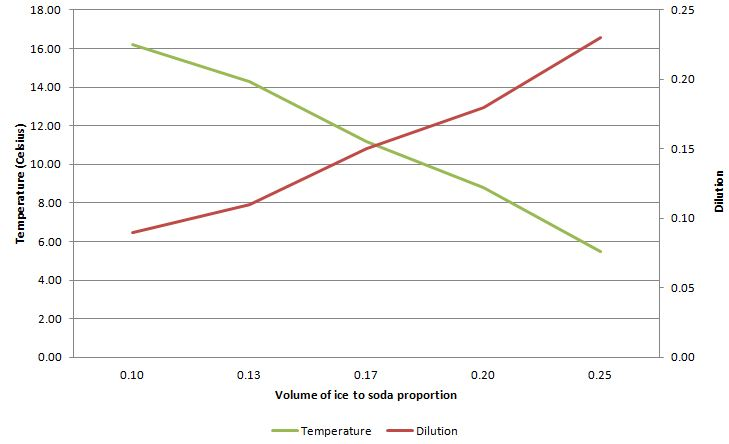
\includegraphics[width=\textwidth]{extra/Graph.jpg}
\end{figure}

\vspace{12pt}
Using the lemmas under Appendix A, we are able to calculate the final temperature and dilution. This is assuming we have the ratio of the volume of ice to soda. This is a different measuring scale from the experimental-based approach. In the experimental-based approach, the percentage is based on the height of a standard regular McDonald's cup. However, in this approach, we are using the ratio as exact absolute volume. Thus, we first calculate how much energy it would take to melt the ice, and see how many degrees it would lower the temperature of the drink by. Then, we calculate what is the temperature that the soda and melted ice would eventually converge to. Also, the dilution is calculated by finding the resulting volume of the melted ice (since ice has a lower density than water), and dividing that by the amount of soda.

Figure 1 is generated by plotting the data from table 12. These basically show a more theoretical approach, which asserts that as more ice is put in the soda, the temperature is further decreased, but the dilution is increased. This take-away from this theoretical result is congruent to those of our experimental results.  This analysis, and the generated trendline, is important because if our sponsor decides on a certain volume of ice to soda proportion and would like to find out the dilution and temperature effects, we can extropolate and further provide the desired calculations. 

%\include{G_Conclusion}

%\ifthenelse{\boolean{@twoside}}{\myclearpage}{}
\prefacesection{Conclusion}

\begin{table}[ h]
\centering
\begin{tabular}{ l || c|c|c }
  &40\% &60\% & 75\%  \\
\hline  
Coke & 61 & 112 & 115 \\
\hline  
Sprite & 31& 59 & 54 \\
\hline  
Fanta Orange & 27 & 58 & 59 \\ 
\hline  
Diet Coke & 15 & 24& 33 \\ 
\hline  
Total & 134 & 253 & 261  \\ 
\hline     
 \end{tabular}
\caption{Experimental Totals}
\end{table}


\vspace{24pt}
Table 13 shows the compiled set of preferences for each soda. To get this table,  we summed up the preferences of each soda at each point in time (t = 0.5, 2, 5, 30 minutes), but taking into account only those data points that are considered significant. This allows us to measure only \emph{clear} trends in the data, and hence scrutinize those specific instances that exhibit an evident preference towards one amount of ice over another. 

\vspace{12pt}
From this table, we can see that across all sodas, there is a clear disinclination towards the cup being filled 40\% with ice. Yet between 60\% or 75\%, there is no clear 'winner' either. However, we know that subjects prefer the cup with more ice if they are to finish their drink quickly, and less ice if they are going to keep the drink for a while. Based on the data and analysis performed \emph{in this experiment alone}, we can conclude that in filling a soda cup, customers, on average, \bf{ prefer a cup filled with 75\% of ice if they intend to drink it in the short term, but prefer a cup filled with 65\% of ice if they intend to drink it in the long term. }

%\include{chapter1}
%\include{chapter2}
%\include{chapter3}
%\include{chapter4}
%\include{chapter5}
%\include{chapter6}


\appendix
\ifthenelse{\boolean{@twoside}}{\myclearpage}{}

\chapter{Lemmas}\label{Lemma}
\vspace{12pt} 

q=mC$\Delta$T,
\\*  where C = specific heat capacity (J/g ºC)
\\* q = quantity of heat in joules 
\\* m = mass in grams
\\* $\Delta$T= change in temperature
\\*  so C= q/(m*$\Delta$ T)

\chapter{Glossary}\label{Glossary}

\vspace{10pt} 

\vspace{8pt}
\noindent {\bf Specific heat capacity}. Amount of heat per unit mass required to raise the temperature by one degree Celsius

\noindent {\bf Heat of fusion}. Amount of heat needed to change its state from a solid to a liquid per unit mass

\ifthenelse{\boolean{@twoside}}{\myclearpage}{}
\chapter{Matlab code}\label{Matlab code}
\begin{lstlisting}[caption= Matlab code for calculating resulting temperature and dilution, label = matlab]

function [dilution, temp] = SHC(vsoda,vice, w )
%vsoda=volume of soda in cm3, Assume density of soda is 1g/cm3
%vice=volume of ice in cm3, Assume density of ice is 0.9167g/cm3
%w=specific heat capacity of soda in J
%specfic heat capacity of water = 4.1813J/g/K
%specific heat of fusion = 334J/g
%Assume ice is 0degrees Celsius, soda is 25 degrees Celsius
%dilution is dilution of resulting solution
%temp is resulting temperature of solution in Celsius

watershc=4.1813;
fusion=334;
density=0.9167;
t=25; %room temperature

vice=vice*density; %find mass of ice
dilution=vice/vsoda; %find dilution
energymelt=334*vice; %find energy needed to melt ice

temp=(t*vsoda*w-energymelt)/(watershc*vice+vsoda*w); %resulting temperature

end
\end{lstlisting}
\vspace{5pt}

\ifthenelse{\boolean{@twoside}}{\myclearpage}{}
\chapter{R code}\label{R}
\begin{lstlisting}[caption= R code for implementing Pearson's chi-squared test, label = Rcode]

x=c(15,25,32)
chisq.test(x)
x=c(14,24,34)
chisq.test(x)
x=c(14,27,31)
chisq.test(x)
x=c(18,36,18)
chisq.test(x)
x=c(15,27,30)
chisq.test(x)
x=c(20, 19, 33)
chisq.test(x)
x=c(14, 29, 29)
chisq.test(x)
x=c(18, 36, 18)
chisq.test(x)
x=c(15,23,34)
chisq.test(x)
x=c(19,23,30)
chisq.test(x)
x=c(18,27,27)
chisq.test(x)
x=c(12,25,35)
chisq.test(x)
x=c(15,24,33)
chisq.test(x)
x=c(21,19,32)
chisq.test(x)
x=c(16,24,32)
chisq.test(x)
x=c(18,22,32)
chisq.test(x)
\end{lstlisting}
\vspace{5pt}
%\endinput

% Add your bibliography to Contents
\ifthenelse{\boolean{@twoside}}{\myclearpage}{\newpage}
\addtocontents {toc}{\protect \contentsline {chapter}{REFERENCES}{}}
\addcontentsline{toc}{chapter}{Selected Bibliography Including Cited Works}  

% Bibliography must come last.
\bibliographystyle{plain}
\renewcommand\bibname{Selected Bibliography Including Cited Works}
\nocite{*}  % List ALL references in your references, not just the ones cited in the text.
% This scheme automatically alphabetizes the Bibliography.
\bibliography{Biblio}
\end{document}
